\FloatBarrier
\section{Các giải pháp kỹ thuật cho luồng nghiệp vụ cốt lõi}
Ba nhóm giải pháp tập trung vào tính nhất quán lịch, quyền tiếp cận và tổ chức dữ liệu. Chúng giải thích cách các bước kiểm tra, trạng thái và ranh giới dữ liệu hỗ trợ luồng nghiệp vụ cốt lõi.

\subsection{Chống trùng lịch, giao dịch và quyết định duyệt}
\label{sec:overlap-solution}
\paragraph{Bài toán.} Hai lượt đặt có thể không trùng khi đọc riêng nhưng xung đột khi cùng được ghi. Cần phân biệt khoảng chạm biên với khoảng giao nhau; đồng thời kiểm lại phòng khi admin duyệt vì lịch bảo trì hoặc lượt đã duyệt có thể thay đổi trong thời gian chờ.

\paragraph{Phép kiểm khoảng.} Với cùng ngày, hai khoảng nửa mở \textit{[s1,e1)} và \textit{[s2,e2)} giao nhau khi đồng thời có \textit{s1 < e2} và \textit{s2 < e1}. Dùng bất đẳng thức chặt nên 08:00--09:00 và 09:00--10:00 được xem là liền kề. Ngày khác nhau không giao trong phép kiểm này. Dữ liệu thời gian được chuẩn hóa và kiểm tra trước phép so sánh; khoảng có giờ bắt đầu lớn hơn hoặc bằng giờ kết thúc bị từ chối.

Nghiệp vụ đặt phòng và bảo trì dùng chung phép kiểm khoảng; backend thực hiện điều kiện tương ứng trong tầng dịch vụ. Khi tạo, hệ thống xét phòng, lịch của chính user và bảo trì; khi duyệt một lượt đang chờ, code kiểm lại thời gian kết thúc, bảo trì và xung đột với lượt đã duyệt của phòng. Kiểm tra khi tạo bảo đảm yêu cầu hợp lệ; kiểm tra khi duyệt bảo đảm quyết định dựa trên lịch và bảo trì hiện thời.

\paragraph{Thứ tự giao dịch ở backend.} \code{BookingService.createBooking} dùng \code{@Transactional}, khóa Configuration và Room bằng \code{PESSIMISTIC_WRITE} trước khi đọc lịch. Với chuỗi lặp, từng lượt được sinh, kiểm và bổ sung vào tập xét để phát hiện cả xung đột trong chuỗi (Bảng~\ref{tab:create-transaction}).
{\tabletext\renewcommand{\arraystretch}{1.04}\begin{longtable}{>{\raggedright\arraybackslash}p{\dimexpr0.12\textwidth-2\tabcolsep\relax}>{\raggedright\arraybackslash}p{\dimexpr0.88\textwidth-2\tabcolsep\relax}}
\caption{Thứ tự tạo booking trong giao dịch Java}\label{tab:create-transaction}\\
\toprule \textbf{Bước} & \textbf{Xử lý}\\\midrule
\endfirsthead
\multicolumn{2}{l}{\small Thứ tự tạo booking trong giao dịch Java (tiếp)}\\
\toprule \textbf{Bước} & \textbf{Xử lý}\\\midrule
\endhead
\bottomrule\endlastfoot
1 & Kiểm actor là user và không mạo danh requesterUsername khác.\\\addlinespace[1.5pt]
2 & Khóa cấu hình chung và bản ghi phòng được chọn trước khi đọc lịch.\\\addlinespace[1.5pt]
3 & Kiểm định dạng ngày và số tuần lặp; sinh ngày của từng lượt nếu đặt theo chuỗi.\\\addlinespace[1.5pt]
4 & Validate từng lượt: phòng, giờ, bảo trì, chồng phòng/user, mục đích, cửa sổ và hạn mức theo điều kiện của lượt đầu/lượt lặp.\\\addlinespace[1.5pt]
5 & Tạo booking với trạng thái ban đầu PENDING; lưu metadata chuỗi và bổ sung vào tập đang xét.\\\addlinespace[1.5pt]
6 & Sau validation, AutoApprovalPolicy quyết định có tự duyệt: chỉ khi công tắc bật và phòng không yêu cầu duyệt riêng.\\\addlinespace[1.5pt]
7 & Nhánh tự duyệt cập nhật APPROVED, người duyệt system, quyền PIN nếu phòng PIN và thông báo; nhánh thủ công giữ PENDING và báo admin.\\\addlinespace[1.5pt]
8 & Trả BookingResult trong giao dịch. Lỗi dữ liệu/điều kiện được ném thành ngoại lệ; không trả kết quả thành công cho lượt vi phạm.\\\addlinespace[1.5pt]
\end{longtable}}

\code{reviewBooking} khóa Configuration và booking đích; khi duyệt sẽ kiểm trạng thái PENDING và các điều kiện hiện thời rồi cập nhật quyết định. Quyền PIN được cấp cho phòng khóa số sau khi duyệt. Sơ đồ trình tự Hình~\ref{fig:sequence-booking} bổ sung điểm gọi qua UI, client HTTP, filter, controller và service; thứ tự khóa và kiểm tra dữ liệu được tổng hợp trong Bảng~\ref{tab:create-transaction}.
\begin{figure}[H]\centering
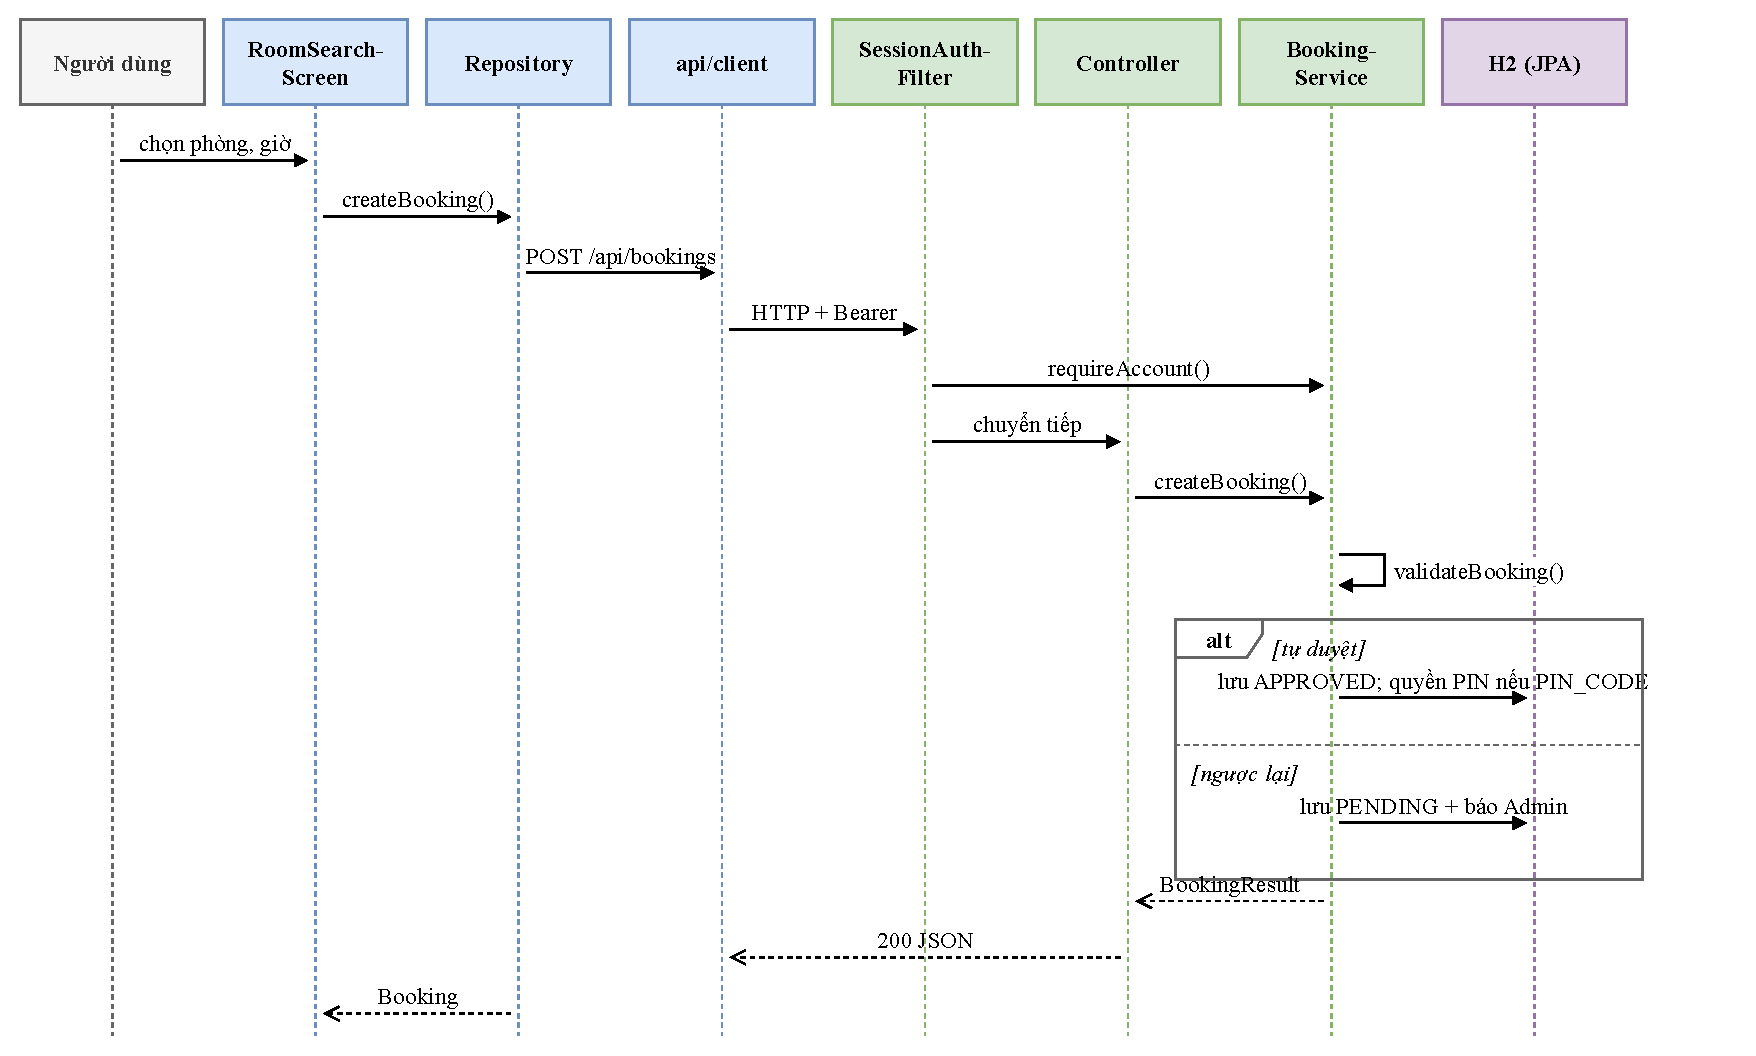
\includegraphics[width=\textwidth,height=.76\textheight,keepaspectratio]{Hinhve/design/15b_sequence_tao_yeu_cau_dat_phong.pdf}
\caption{Trình tự tạo booking qua REST và nhánh tự duyệt/thủ công}\label{fig:sequence-booking}
\end{figure}

\paragraph{Kết quả và hạn chế kỹ thuật.} Các ca kiểm thử ở Chương~\ref{chap:testing} xác nhận xử lý đúng trùng lịch, chạm biên, bảo trì và hạn mức. Backend khóa bản ghi cấu hình/phòng trước khi kiểm và ghi dữ liệu. Khóa cấu hình chung khiến các thao tác dùng cùng tài nguyên phải chờ nhau, là điểm cần tối ưu khi mở rộng. Kho local đọc/ghi JSON, còn backend quản lý giao dịch và khóa dữ liệu bằng JPA.

\FloatBarrier
\subsection{Cấp quyền theo phòng và vòng đời PIN tạm thời}
\label{sec:pin-solution}
\paragraph{Bài toán.} Vai trò user không được biến thành quyền tạo mã ở mọi phòng. Một người chỉ được tạo PIN cho booking đã duyệt của mình, tại phòng được phép và đang gắn khóa phù hợp. Kết nối OneIoT có thể chưa có khi tạo mã, vì vậy lưu mã và gửi lệnh cần là các trạng thái riêng.

\paragraph{Kiểm quyền ở các tầng.} Dịch vụ cấp PIN kiểm vai trò, booking tồn tại/APPROVED, phòng PIN, chủ lượt/quyền theo phòng đối với user, chưa có PIN chưa thu hồi và lượt chưa kết thúc. Admin có quyền thao tác phù hợp nhưng vẫn phải đáp ứng các điều kiện nghiệp vụ của booking/phòng. Khi duyệt tay hoặc tự duyệt phòng PIN, hệ thống cấp quyền cho cặp username--roomId. Thu hồi quyền theo phòng tách khỏi thay đổi role tài khoản.

Mã mới chỉ được tạo khi lượt đặt không còn PIN chưa thu hồi. Do đó, PIN hết thời gian nhưng chưa ghi nhận thu hồi vẫn ngăn việc cấp mã tiếp theo.

\paragraph{Khoảng hiệu lực và ID khóa.} Mã nghiệp vụ có đúng bảy chữ số. Với khoảng sử dụng, validFrom được tính bằng giờ bắt đầu trừ khoảng đệm; validUntil bằng giờ kết thúc cộng khoảng đệm. Giá trị mặc định là 10 phút và đọc từ cấu hình, không gắn cứng trong UI. Trước khi lưu, service xin password ID của khóa gắn phòng; ID nằm trong 1--255 và quay vòng sau 255. Backend khóa bản ghi khóa khi cấp ID. Cấp ID, lưu PIN và gửi MQTT là các lời gọi riêng trong quy trình.

\paragraph{Lưu trước, gửi khi có phiên.} App lưu code, thời hạn và password ID vào booking trước. Nếu OneIoT chưa nối, người dùng vẫn xem được mã và trạng thái chờ. Khi có phiên, \code{deliverPendingTemporaryPins} duyệt các PIN chưa thu hồi/chưa gửi, booking còn APPROVED, đúng phòng đang gắn khóa và chưa hết hạn. Một lần gửi thất bại được ghi thông tin lần thử/lỗi để UI phân biệt với chưa thử gửi.

\begin{figure}[H]\centering
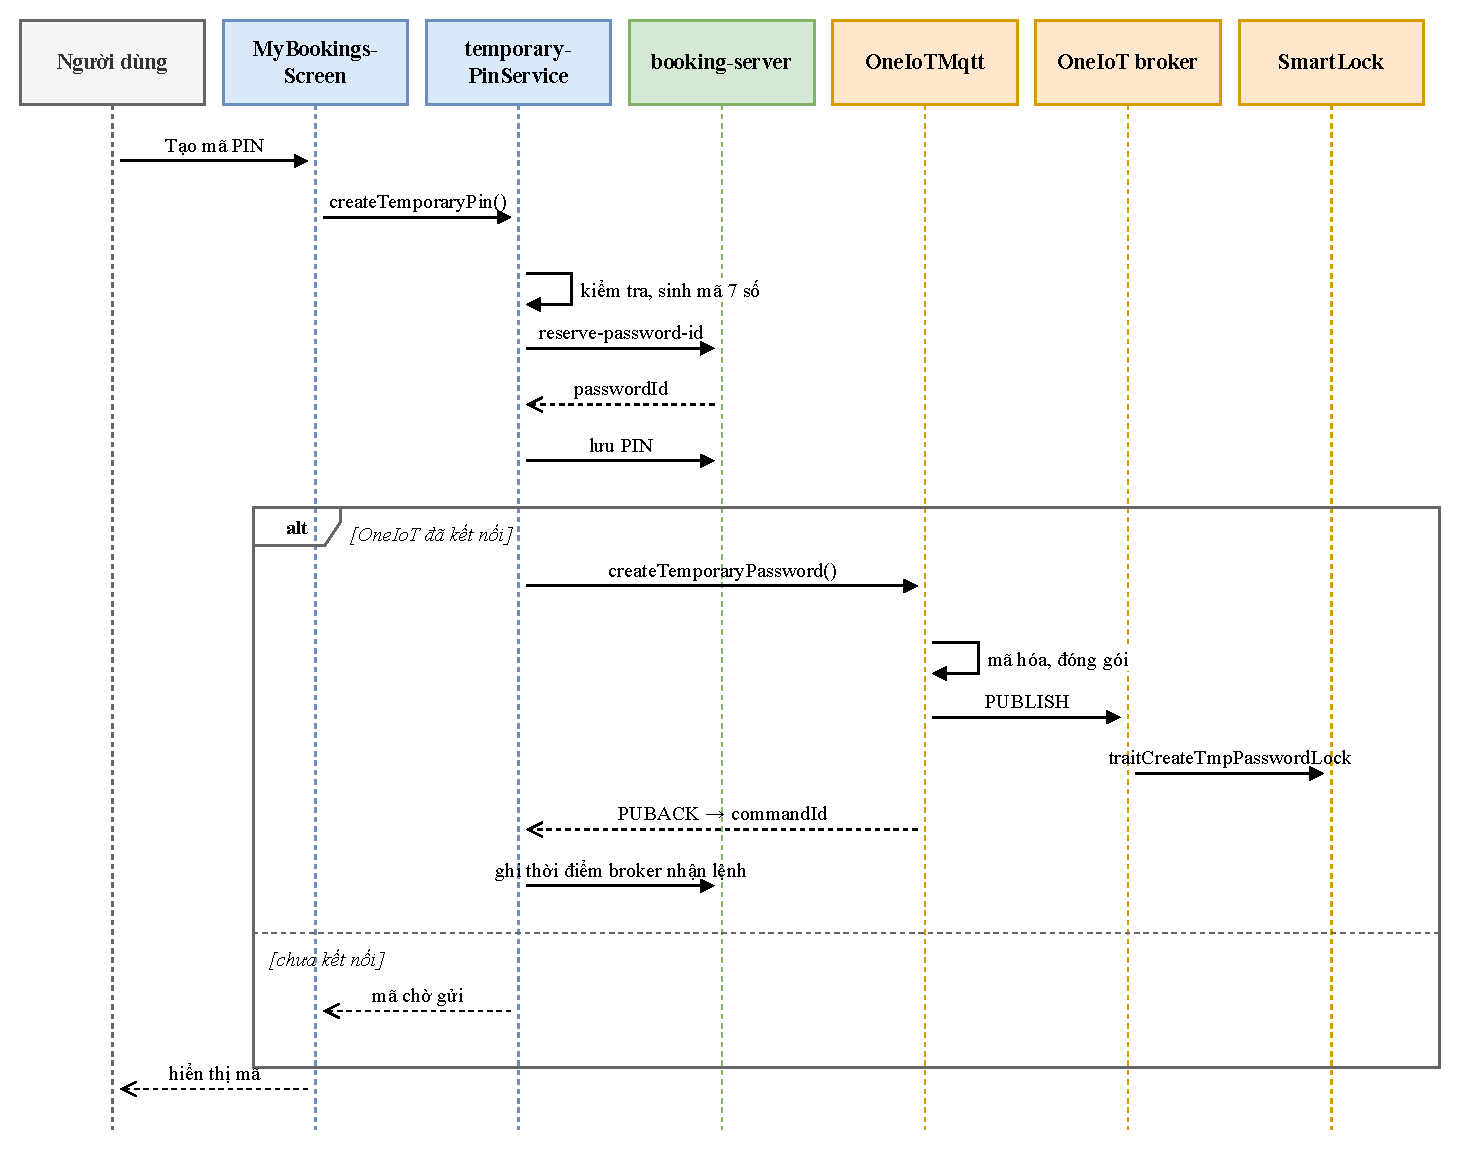
\includegraphics[width=\textwidth,height=.76\textheight,keepaspectratio]{Hinhve/design/16a_sequence_tao_pin_tam.pdf}
\caption{Tạo, lưu và gửi PIN; xác nhận publish của broker tách với thực thi trên khóa}\label{fig:sequence-pin}
\end{figure}

Native \code{OneIoTMqttPackage.kt} chuyển thời hạn sang định dạng bản tin, mã hóa phần mật khẩu và gửi trait \code{traitCreateTmpPasswordLock}. Sau publish được broker xác nhận, app lưu \code{lockDeliveredAt} và request ID. Giao diện cập nhật trạng thái gửi theo kết quả publish; các bản tin sự kiện khóa được xử lý qua luồng nhận MQTT.

\paragraph{Kết quả và hạn chế kỹ thuật.} Các kiểm thử access control và native bridge xác nhận đúng dữ liệu, quyền, thời hạn và cơ chế gửi lại. Ứng dụng và SmartLock thực hiện luồng cấp, sử dụng PIN thực tế. Trạng thái revokedAt quản lý PIN trong booking. Hướng gia cố gồm quản lý ID hữu hạn, bảo vệ dữ liệu, nguồn sinh mã và phản hồi thiết bị.

\FloatBarrier
\subsection{Cùng giao diện nghiệp vụ, hai chế độ dữ liệu}
\label{sec:two-data-solution}
\paragraph{Bài toán.} Hệ thống hỗ trợ vận hành độc lập trên một thiết bị và sử dụng dữ liệu dùng chung qua REST. Hai chế độ dùng cùng giao diện nghiệp vụ để giảm lặp xử lý; nguồn dữ liệu được chọn rõ ràng trong cấu hình bản build.

\paragraph{Giải pháp triển khai.} Repository giữ các hàm nghiệp vụ mà UI gọi; \code{isRemoteApiEnabled} chọn nhánh REST hoặc đọc/ghi JSON local. Client tập trung thêm token và chuyển lỗi mạng/HTTP thành Error cho màn hình. Kiểu TypeScript và cấu trúc request/response Java xác định hợp đồng trao đổi; kiểm thử API kiểm tra phương thức, dữ liệu, phiên và các nhánh lỗi.
{\tabletext\renewcommand{\arraystretch}{1.04}\begin{longtable}{>{\raggedright\arraybackslash}p{\dimexpr0.22\textwidth-2\tabcolsep\relax}>{\raggedright\arraybackslash}p{\dimexpr0.37\textwidth-2\tabcolsep\relax}>{\raggedright\arraybackslash}p{\dimexpr0.41\textwidth-2\tabcolsep\relax}}
\caption{Đối chiếu thao tác local và REST}\label{tab:local-remote}\\
\toprule \textbf{Thao tác} & \textbf{Local} & \textbf{REST}\\\midrule
\endfirsthead
\multicolumn{3}{l}{\small Đối chiếu thao tác local và REST (tiếp)}\\
\toprule \textbf{Thao tác} & \textbf{Local} & \textbf{REST}\\\midrule
\endhead
\bottomrule\endlastfoot
Xác thực & Đọc tài khoản của kho thiết bị, tạo session UI. & Login tạo token/actor tại server; request sau mang Bearer.\\\addlinespace[1.5pt]
Tạo/duyệt booking & Repository kiểm quy tắc trên các tập dữ liệu local và ghi JSON. & API/service kiểm actor và dữ liệu trong giao dịch; server là nơi quyết định trạng thái được lưu.\\\addlinespace[1.5pt]
Phòng/cấu hình/bảo trì & Mỗi máy giữ danh mục và cấu hình riêng. & Các client gọi cùng server sử dụng chung danh mục, cấu hình và dữ liệu phòng.\\\addlinespace[1.5pt]
Quyền và PIN & Quyền và PIN gắn tài khoản/phòng/booking trong kho local. & Quyền và PIN lưu ở server; việc gửi MQTT vẫn xuất phát từ app/native, không chuyển cho Java.\\\addlinespace[1.5pt]
Thông báo & Lưu theo người nhận trong thiết bị; banner chỉ hiện cho tài khoản đang đăng nhập. & Server lưu theo user; client tải thông báo qua REST bằng phiên đăng nhập.\\\addlinespace[1.5pt]
Lỗi kết nối & Không cần booking server; OneIoT vẫn là kết nối riêng nếu dùng khóa. & Trả lỗi/timeout theo client; không tự fallback hoặc tải backlog local.\\\addlinespace[1.5pt]
\end{longtable}}

\paragraph{Kết quả và hạn chế kỹ thuật.} Một nhóm màn hình phục vụ cả hai chế độ; thay đổi cấu hình chọn nguồn dữ liệu mà không chuyển dữ liệu giữa hai kho. Nếu bổ sung offline sync sau này, cần thiết kế định danh, hàng đợi, phiên bản dữ liệu, quy tắc hòa giải và kiểm thử độc lập. Kiểm thử hợp đồng REST duy trì cấu trúc trao đổi giữa app và server; khi mở rộng cần quản lý kết nối, tính sẵn sàng của dịch vụ và dữ liệu dùng chung.
